\documentclass{article}

% if you need to pass options to natbib, use, e.g.:
% \PassOptionsToPackage{numbers, compress}{natbib}
% before loading nips_2017
%
% to avoid loading the natbib package, add option nonatbib:
% \usepackage[nonatbib]{nips_2017}

%\usepackage{nips_2017}

% to compile a camera-ready version, add the [final] option, e.g.:
\usepackage[final]{nips_2017}

\usepackage[utf8]{inputenc} % allow utf-8 input
\usepackage[T1]{fontenc}    % use 8-bit T1 fonts
\usepackage{hyperref}       % hyperlinks
\usepackage{url}            % simple URL typesetting
\usepackage{booktabs}       % professional-quality tables
\usepackage{amsfonts}       % blackboard math symbols
\usepackage{nicefrac}       % compact symbols for 1/2, etc.
\usepackage{microtype}      % microtypography
\usepackage{graphicx}
\usepackage{color}

\newcommand{\yuqing}[1]{\textcolor{red}{(Yuqing: #1)}}

\title{Lung Cancer Detection from CT Scan Images Using Deep Convolutional Neural Networks}

% The \author macro works with any number of authors. There are two
% commands used to separate the names and addresses of multiple
% authors: \And and \AND.
%
% Using \And between authors leaves it to LaTeX to determine where to
% break the lines. Using \AND forces a line break at that point. So,
% if LaTeX puts 3 of 4 authors names on the first line, and the last
% on the second line, try using \AND instead of \And before the third
% author name.

\author{
  Yuqing Zhang$^1$ \quad Rahul Bazaz$^2$ \quad Howard Fan$^1$ \quad Maulik Shah$^3$ \\
  $^1$Graduate Program in Bioinformatics \\ $^2$Undergraduate Program in Computer Science \& Business Admin \\ $^3$Graduate Program in Computer Science \\
  Boston University, Boston, MA 02215 \\
  \texttt{\{yuqingz, rbazaz, hjfan, maulikjs\}@bu.edu} \\
}

\begin{document}
% \nipsfinalcopy is no longer used

\maketitle

\begin{abstract}
Deep Convolutional Neural Networks (DCNNs) are the key ingredient in the recent progress in computer vision, medical image processing, and many other machine learning areas. In this project, we participated in the Data Science Bowl 2017 (DSB-17) challenge \cite{dsb17} on lung cancer detection. We built a lung cancer detection model based on deep convolutional neural networks to predict from CT scan images whether a patient has lung cancer. 
To build an effective model for this task, one needs to address several challenges. First, the raw CT scan images need to be preprocessed to extract the lung regions of interest. Second, compared with the typical use-case of deep convolutional neural networks on two-dimensional images, CT scan images are three-dimensional and require significantly more computational resources, imposing restrictions on network architecture and training batch size. Third, the limited size of the provided DSB-17 dataset also introduces difficulties and risks of overfitting in training deep convolutional neural networks.
To handle the above challenges, we explored different model designs and techniques, and used LUNA-16 as our external dataset. 
In the end, we achieved (after the challenge deadline) 0.55 loss and 76.7\% accuracy on the DSB-17 test set, which is comparable to the top-50 performances on the Data Science Bowl leader-board.
\end{abstract}

\section{Introduction}
\label{sec:intro}

As lung cancer causes 1.6 million deaths every year around the world \cite{stewart2014world},  lung cancer detection and diagnosis is crucial for health care. An increasing amount of research effort has been devoted to building automatic systems for lung cancer detection based on machine learning. The Data Science Bowl 2017 (DSB-17) \cite{dsb17} holds a challenge for lung cancer detection. This challenge requires building a binary classification system that takes the CT scan images of the patients as the input and predicts a probabilistic classification result indicating whether the patient has cancer or not.

In this project, we address the lung cancer detection task in the DSB-17 with Deep Convolutional Neural Networks (DCNNs), which are the key components in state-of-the-art methods in computer vision, medical image processing, and many other areas. They are neural networks that involve several convolutional layers, followed by densely connected (i.e. fully connected) layers. DCNNs are proven to be powerful in both image-level classification and pixel-wise segmentation.

To apply deep convolutional neural networks to our cancer detection task, we need to handle several issues in both machine learning and computation. The first issue is data limitation. It is well known that deep convolutional neural networks typically require a large amount of data (``big data'') to train. For example, the ResNet model \cite{he2016deep} for 2D image classification in computer vision is trained on 14 million images. However, compared to abundant natural images over the Internet, medical images such as CT scans or fMRI images are much more expensive to collect. Consequently, it is difficult or even impossible to obtain large-scale datasets of medical images that have a comparable size as in those ``big data'' areas. In the DSB-17 dataset for lung cancer detection, there are only 1397 patients available for training, and each patient is associated with only one CT scan image plus a binary label indicative of cancer. This Data Science Bowl dataset is two or three magnitudes of order smaller compared to typical large-scale datasets used to train deep convolutional neural networks in computer vision \cite{deng2009imagenet,lin2014microsoft}. Even though we incorporate the external LUNA-16 dataset \cite{setio2016validation}, our total number of patients is still below 2000. The lack of large-scale datasets poses a great challenge in applying deep convolutional neural networks on this task.

Besides the data limitation, computation cost is another obstacle in applying deep convolutional neural networks for lung cancer detection. Compared to traditional machine learning models such as support vector machines, neural networks requires considerably more computation resources, and are often deployed in parallel computing hardware such as GPUs. Moreover, the CT images are three-dimensional rather than two-dimensional. In order to process them, we need three-dimensional convolutional operations in the network instead of the (more often used) two-dimensional convolutional operations. Hence, it takes significantly more time to perform forward and backward propagation and more GPU memory to store the network and intermediate computation results. The higher computation cost and memory consumption mean that for a given time, one can only train for a fewer number of iterations. And for a given GPU memory budget, one can only put in a small number of samples in a batch. The latter (a small batch size) may cause problems in neural network training: as deep convolutional neural networks are typically trained based on mini-batch gradient descent that estimates the gradient of the loss function on the entire dataset using a batch of samples, a small batch size means that the gradient on each batch can be noisy, so the training procedure may fail to converge.

Apart from the data limitation, computation cost, and memory consumption, the preprocessing method also affects the overall performance of lung cancer detection and poses further challenges. Deep convolutional neural networks often require the inputs to have the same shape. However, different CT scan images may have different shapes (lengths, widths, and heights) and spacing (the actual distance in millimeters between two adjacent voxels in the 3D CT scan images). So one needs to decide how to unify them to the same shape, in order to feed them into the same network. One also needs to balance the trade-off between the input shape and the computation cost. Over-sized inputs may consume too much memory, while trimming the images too small may reduce resolution and lose useful information. Also, for lung cancer detection, only the lung region in the CT scan is of interest to the task, so one needs an approach to segment the lung regions in the CT scans and remove the other regions during preprocessing. We describe our preprocessing procedure in Sec. \ref{sec:preprocssing}.

When trying to build a lung cancer detection model with deep convolutional neural networks, we encountered all the issues above. In our first method described in Sec. \ref{sec:method1}, we used a large input shape and could only use a very small batch size of 3 to fit into our Nvidia Tesla K40 GPU. Under this setting, the training procedure based on mini-batch gradient descent failed to converge. After switching to a new preprocessing setting that results in a smaller input size, we could raise our batch size to 64. However, severe overfitting occurred: we got a 100\% accuracy on the training set, but only 71.2\% on the test set which is equivalent to the accuracy of classifying all samples as negative. We tried to combat overfitting by adding more regularization and reducing model complexity. However, while we were able to bring down the accuracy on the training set with higher regularization and simpler models, we were unable to make it work better than 71.2\% on the test set.

This motivated us to add more data for training. We first tried a simple data augmentation technique of taking random crops from the 3D CT scans, which did not work well. Then we decided to incorporate the LUNA-16 dataset for lung nodule detection to get more training data. As the LUNA-16 dataset contains different annotations from our main dataset DSB-17, we took a different training procedure in Sec. \ref{sec:method2}. We first trained a nodule segmentation model based on U-Net \cite{ronneberger2015u} to segment the nodules in the CT scans, and then classified each patient based on his/her top-20 nodule candidates. In this way, we eventually achieved a loss of 0.55 and an accuracy of 76.7\% on the test set (after the challenge deadline), which is comparable to the top-50 in the Data Science Bowl 2017 leader-board.

\section{Background and datasets}
\label{sec:background}

\paragraph{CT scan images}
Our lung cancer detection task is based on CT scan images over the patients' lung regions. Each CT scan image is a three-dimensional data array (or equivalently, a 3D image) with one channel at each voxel. The elements in the array (i.e. voxels in the 3D image) contain the Hounsfield Units (HU) that measure the radiodensity at each location. Different substances in the lung region have different HU values, so the CT scan image reveals the structure (such as the presence of tumors) inside the lung region. Figure \ref{fig:ct_scan} shows an example image, and Table \ref{tab:hu_values} contains the HU values of typical substances in human body. Due to the different settings of the scanning machines, different CT images may have different shapes and spacing. They need to be unified before further processing.

\begin{figure}[t]
  \centering
  \begin{tabular}{ccc}
  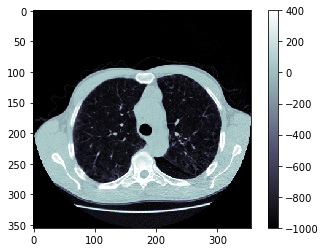
\includegraphics[height=100px]{figures/dsb17_1.png} &
  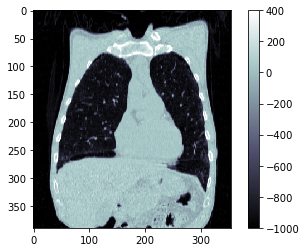
\includegraphics[height=100px]{figures/dsb17_2.png} &
  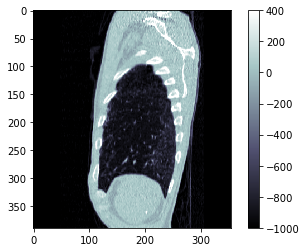
\includegraphics[height=100px]{figures/dsb17_3.png} \\
  (a) & (b) & (c) \\
  \end{tabular}
  \caption{An example CT scan image in the DSB-17 dataset, showing the slices of the 3D image and the HU values along (a) $z$-axis, (b) $y$-axis and (c) $x$-axis respectively.}
  \label{fig:ct_scan}
\end{figure}

\begin{table}[t]
  \begin{center}
  \begin{tabular}{ll|ll|ll}
    \toprule
    Substance & HU & Substance & HU & Substance & HU \\
    \midrule
    Air & -1000         & Lung & -500 & Fat & -120 to -90 \\     Water & 0  & Urine & -5 to +15   & Bile & -5 to +15 \\
    CSF & +15          & Kidney & +20 to +45 & Lymph nodes    & +10 to +20 \\
    Blood & +30 to +45 & Muscle & +35 to +55 & Grey matter & +37 to +45 \\
    White matter & +20 to +30 & Liver & +40 to +60 & Soft Tissue, Contrast & +100 to +300 \\
    Bone & +700 to +3000 & Chyle & -30 \\
    \bottomrule
  \end{tabular}
  \end{center}
  \caption{The typical Hounsfield Units (HU) of substances in human body.}% The HU values of the lung (including the air in the lung) is within the range $-1000$ to $+400$.}
  \label{tab:hu_values}
\end{table}

\paragraph{Lung cancer detection and the Data Science Bowl 2017 dataset}
Lung cancer is a disease that involves \textit{malignant} nodules in patients' lungs. The term \textit{nodule} represents a spectrum of abnormalities in the lung that may represent primary lung cancers, metastatic disease, or non-cancerous processes. In other words, only the patients with nodules in their lungs can potentially have cancer, while not all nodules indicate lung cancer. Having lung nodules is a \textit{necessary but not sufficient condition} for having lung cancer.

The Data Science Bowl 2017 (DSB-17) dataset \cite{dsb17} consists of 1595 patients, including 1397 for training (362 cancer and 1035 non-cancer) and 198 for test/evaluation (57 cancer and 141 non-cancer). Each patient is associated with a 3D CT scan image and a cancer/non-cancer binary label. The task is to train on the training split and evaluate on the test split through the provided evaluation server. It is allowed to evaluate multiple times on the test split and take the best score.

\paragraph{Nodule segmentation and the LUNA-16 dataset}
The LUNA-16 dataset \cite{setio2016validation} is used as our external dataset to train a nodule segmentation model in Sec. \ref{sec:method2}. This dataset also contains CT scan images of the patients' lung regions. However, unlike DSB-17 that contains binary cancer/non-cancer labels, the LUNA-16 dataset contains \textit{the sizes and locations of nodules} in each patient. There are 601 CT scan images in the LUNA-16 dataset, and all the nodules present in each image are labeled with the X, Y and Z coordinates and diameters.

The original task on the LUNA-16 dataset is nodule segmentation, that is, predicting the locations and sizes of all nodules in a given 3D CT scan image. Figure \ref{fig:luna16_data} shows an example CT scan and its nodule annotation in LUNA-16.

\begin{figure}[t]
  \centering
  \begin{tabular}{cc}
  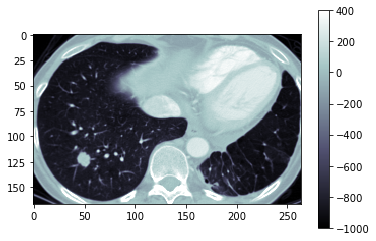
\includegraphics[height=100px]{figures/luna16_1.png} &
  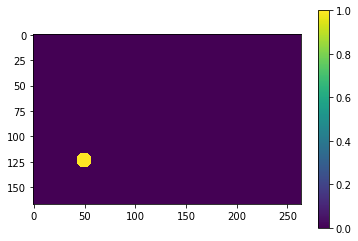
\includegraphics[height=100px]{figures/luna16_2.png} \\
  \end{tabular}
  \caption{A example CT image in the LUNA-16 dataset. Left: one slice of CT scan along $z$-axis. Right: the corresponding annotated nodule mask (the yellow circular region) for that slice.}
  \label{fig:luna16_data}
\end{figure}

\paragraph{Deep convolutional neural networks}
Deep convolutional neural networks are statistical learning models that have led to recent breakthroughs in many machine learning areas. They are a special kind of neural networks that consists of several \textit{convolutional layers} and \textit{pooling layers}, followed by \textit{densely connected layers} (also called \textit{fully connected layers}). Convolutional layers preserve the spatial structure of the input data, and pooling layers introduce local translation invariance. Like other neural networks, convolutional neural networks can be trained with back-propagation, and are often implemented on GPUs instead of CPUs due to their high computation demand. A thorough review of convolutional neural networks is beyond the scope of this paper, and we refer readers to \cite{Goodfellow-et-al-2016} for a detailed survey of them.

%Since natural images taken from cameras are two-dimensional, the most frequently used deep convolutional neural networks in computer vision involves 2D convolution operations. However, CT scan images are three-dimensional, and it is natural to use 3D convolution \cite{ji20133d} to process these data, resulting in higher computation and memory demand.

\section{Data preprocessing}
\label{sec:preprocssing}
Before feeding the CT scan images into our deep convolutional neural network, we need to unify the spacing of the 3D CT scans, and then segment the lung region from these CT scans. In our experiments, we resize all the CT scans to the same spacing of 1mm (a commonly used spacing in CT image processing) with spline interpolation \cite{spline_interpolation} implemented by the function \verb|scipy.ndimage.interpolation.zoom| in Python. The resized CT scan images have the same spacing: each voxel in the image corresponds exactly to a 1mm $\times$ 1mm $\times$ 1mm cubical region. However, after resizing, different CT scan images may still have different shapes (i.e. lengths, widths, and heights), which we address with different approaches in Sec. \ref{sec:method1} and \ref{sec:method2}.

\paragraph{Lung region segmentation}
After unifying the spacing, we segment the lung regions from the CT scan images. Following \cite{full_preprocssing_tutorial}, the lung region are segmented by finding the largest connected components.

From Table \ref{tab:hu_values}, we see that the lung tissues have HU values around -500, and the air in the lung have HU values around -1000. So the HU values of the entire lung region should be approximately no higher than -500, while the bone regions are usually above 700. To separate the lung from the skeleton, we obtain a 3D binary mask by thresholding the 3D CT scan image at -320: all the voxels with HU values below -320 are labeled as 1 (indicating potential lung regions), and 0 otherwise. Then, we find the largest connected component in the 1 voxels in the binary mask. A voxel is considered to be connected to another voxel if they are adjacent to each other and both have values 1 in the mask. In this way, the CT scan image can be divided into multiple connected components according to voxel connectivity. The largest connected component is the one with the maximum number of voxels in it, which can be obtained using the function \verb|skimage.measure.label| in Python. This largest connected component should cover most of the lung region, and we treat it as the binary mask of the lung.

To also include some tissues around the lung that may contain information relevant to the cancer status, we dilate the largest connected component via a binary erosion \cite{erosion_morphology}, extending the lung mask by 5mm in all directions. Then we apply the dilated lung mask to the original CT scan image by keeping the regions inside the mask and setting all voxels outside the mask to have -1000 HU. Figure \ref{fig:lung_segmentation} shows an example CT scan image and its segmented lung region, from which it can be seen that the obtained segmentation mask corresponds exactly to the lung region.

Since the lung regions we are interested in have HU values in the range -1000 to +400 (all substances above +400 are bones with different radiodensity), after segmenting the lung regions, we set all HU values below -1000 as -1000 and those above +400 as +400, and then linearly rescale the range from -1000 to +400 into the interval from 0 to 1.

\begin{figure}[t]
  \centering
  \begin{tabular}{ccc}
  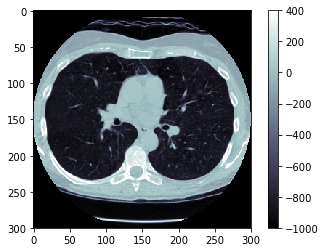
\includegraphics[height=100px]{figures/lung_seg_1.png} &
  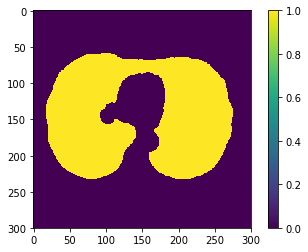
\includegraphics[height=100px]{figures/lung_seg_2.png} &
  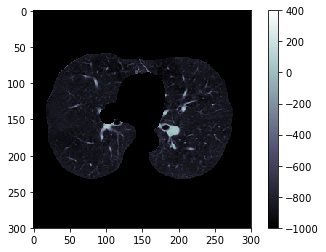
\includegraphics[height=100px]{figures/lung_seg_3.png} \\
  (a) & (b) & (c) \\
  \end{tabular}
  \caption{A sample slice of a CT image, sliced along the $z$-axis. (a) original CT scan image with HU values shown in the color bar. (b) the lung mask obtained from the largest connected component. (c) the segmented lung region after applying the lung mask to the CT image.}
  \label{fig:lung_segmentation}
\end{figure}

\section{Classification Method 1: using a single 3D convolutional neural network}
\label{sec:method1}

\begin{table}[t]
  \begin{center}
  \begin{tabular}{ccccc}
    \toprule
    Layer & Kernel size & Kernel stride & Output channels & Activation function \\
    \midrule
    conv1 & (3, 3, 3) & (1, 1, 1) & 48 & Rectified Linear Unit (ReLU) \\
    conv2 & (3, 3, 3) & (1, 1, 1) & 48 & Rectified Linear Unit (ReLU)\\
    pool2 & (2, 2, 2) & (2, 2, 2) & 48 & - \\
    conv3 & (3, 3, 3) & (1, 1, 1) & 64 & Rectified Linear Unit (ReLU) \\
    conv4 & (3, 3, 3) & (1, 1, 1) & 64 & Rectified Linear Unit (ReLU) \\
    pool4 & (2, 2, 2) & (2, 2, 2) & 64 & - \\
    conv5 & (3, 3, 3) & (1, 1, 1) & 96 & Rectified Linear Unit (ReLU) \\
    conv6 & (3, 3, 3) & (1, 1, 1) & 96 & Rectified Linear Unit (ReLU) \\
    pool6 & (2, 2, 2) & (2, 2, 2) & 96 & - \\
    dense7 & - & - & 256 & Rectified Linear Unit (ReLU) \\
    dense8 & - & - & 1 & no activation (linear activation) \\
    \bottomrule
  \end{tabular}
  \end{center}
  \caption{The 3D convolutional neural network in our Classification Method 1. The network consists of six 3D convolutional layers (with 3 max-pooling layer between them), followed by two densely connected layers.}
  \label{tab:convnet_1}
\end{table}

After preprocessing the data and segmenting the lung regions from the CT scan images, we need to build a binary classification system to classify the images into either cancer or non-cancer. In our experiments, we tried two different methods for classification. In this section, we describe our first method (\textbf{Classification Method 1}) that directly classifies the CT images with a single 3D convolutional neural network.

We design a 3D convolutional neural network that consists of eight parameterized layers, including six \textit{3D convolutional layers} (with three \textit{max-pooling layers} between them) followed by two \textit{densely connected layers} (also called \textit{fully connected layers}). The architecture of this network is summarized in Table \ref{tab:convnet_1}. The rationale behind this design is that the six convolutional layers extract low-level to high-level semantic information from the CT images, then the two densely connected layers act like an ordinary neural network to classify the convolution outputs into the two classes.

Also, we note that in Table 2, lower layers have higher spatial resolutions but fewer channels, while upper layers have lower spatial resolutions but more channels, which is a trade-off for computation cost and memory consumption: we cannot afford to put in more channels in lower layers since their spatial size is already very large (otherwise the network cannot fit into the memory). For each input CT image, the network outputs a scalar score, and we use a sigmoid cross entropy loss over the score as follows
\begin{equation}
\label{eqn:loss}
L = - y \cdot \log \left( \frac{1}{1 + \exp(-s)} \right) - (1 - y) \cdot \log \left(1 - \frac{1}{1 + \exp(-s)}\right)
\end{equation}
where $s$ is the output score from the network and $y$ is the 0/1 binary label for the CT scan image. We implemented this network using the open-source TensorFlow package \cite{abadi2016tensorflow}. The entire network can be trained via back-propagation and mini-batch gradient descent. %by putting a few samples in a batch, calculating the gradient of the loss function on the batch, and use the gradient to update the parameters in the network. 
We use the ADAM solver \cite{kingma2014adam} for parameter update, which is a variant of mini-batch gradient descent that involves momentum and gradient scaling. This network is trained on the training split of the DSB-17 dataset on a machine with a Nvidia K40 GPU.

Since the densely connected layers in Table \ref{tab:convnet_1} require fixed input dimensions, the above network requires that the input shapes (lengths, widths, and heights) are the same over all samples. Hence, we need to normalize the shapes of the CT scans before feeding them into the network. Here, we run into the computation cost and memory consumption issues described in Sec. \ref{sec:intro}. Initially, we took the shape of the largest segmented lung region among the CT images as the network input shape, and padded the smaller lung regions with zeros on each side. This approach kept the 1mm spacing and preserved as much information as possible, but resulted in an input shape of (208, 168, 205), a large size for 3D convolutions. To fit the network with this input shape into the 12GB memory of our Nvidia K40 GPU, we could only use a  small batch size of 3 in our mini-batch gradient descent. We observed that our training is unable to converge with this small batch size, and the loss stayed as high as 0.6 during training. The network trained in this way underfitted the training data and only learned to classify every CT scan image as negative (non-cancer). The resulting accuracy on the training and the test set were 74.1\% and 71.2\%, which are both equal to the fraction of the negative class.

We found that the main reason for the underfitting above is that our batch size 3 is too small. Consequently, the gradients on the mini-batch are noisy and do not reflect the gradient on the entire dataset. To fix this underfitting issue, it was necessary to reduce the computation cost and memory consumption with a smaller input shape, so that a larger batch size could be used. So we took another approach to unify the shape of CT scan images in DSB-17 and resized all images to shape $64\times 64 \times 64$. After this, the network took much less memory with the new input shape, so we could use a much larger batch size of 64 in our mini-batch gradient descent.

However, we found that the network trained in this way severely overfitted the training set. We were able to get nearly 100\% accuracy on the training set, but still 71.2\% accuracy on the test set as before. To combat overfitting, we first tried to add more  regularization, including 1) using a higher L2-regularization over the parameters, 2) adding a dropout layer \cite{krizhevsky2012imagenet} between the two densely connected layers, and 3) adding batch normalization \cite{ioffe2015batch} after each convolutional layer. However, we failed to get any accuracy higher than 71.2\% on the test set using these methods. After diagnosis, we found that the reason for this overfitting behavior was that the training set from DSB-17 has too few samples (1397) compared to our network complexity. 

We then tried to use data augmentation techniques to obtain more data. Instead of using the entire $64\times 64 \times 64$ images after resizing, we randomly took $54\times 54 \times 54$ crops from it at each time when feeding the data into the network, which is a technique commonly used in image classification \cite{krizhevsky2012imagenet}. However, even with data augmentation, the network still overfitted severely. We believed the reason is that, because the crops were highly correlated (since they are cropped from the same image), the effective sample size was not much larger than before. Therefore, it is necessary to increase the number of \textit{actual} patient samples and add external training data to combat overfitting. We added LUNA-16 dataset as our external dataset and developed a new classification approach in Sec. \ref{sec:method2}.

\section{Classification Method 2: cancer prediction based on nodule segmentation}
\label{sec:method2}

We use the LUNA-16 dataset \cite{setio2016validation} as our external data to alleviate the data limitation issue of DSB-17. As the CT scan images in LUNA-16 are annotated with nodule locations and diameters rather than patient-level cancer/non-cancer labels, we cannot simply put LUNA-16 together with DSB-17. We need a new training approach to utilize both datasets. Inspired by \cite{no7}, we developed our second training method (\textbf{Classification Method 2}). Our second method first uses the LUNA-16 dataset to train a nodule segmentation model, then applies it to the CT images in DSB-17 to find candidate nodules, and finally uses a 3D convolutional neural network over the top nodule candidates (instead of the entire image) in DSB-17 to predict patient-level cancer probabilities.

\subsection{Nodule segmentation based on U-Net structure}
\label{sec:nodule_seg_unet}

\begin{figure}[t]
  \centering
  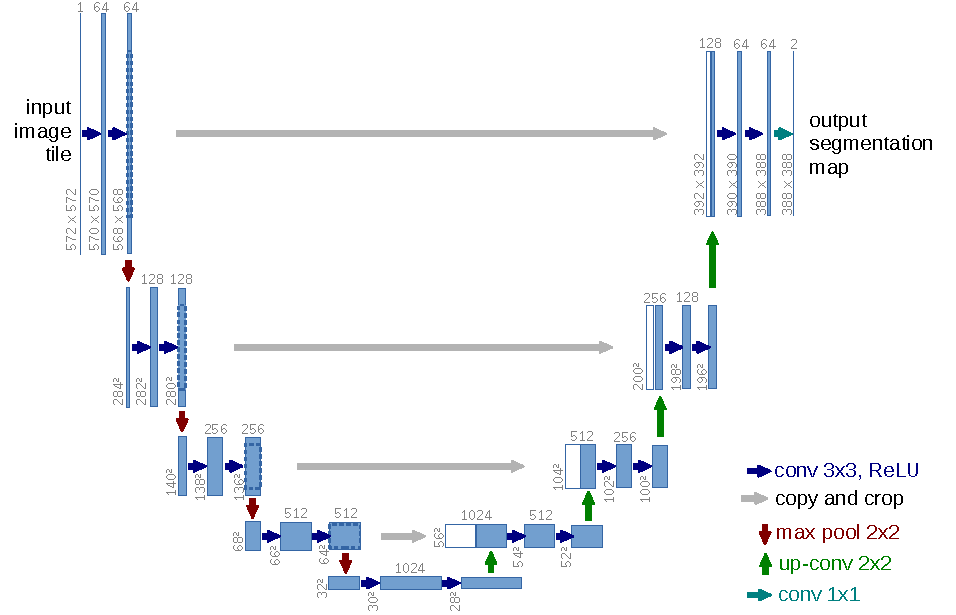
\includegraphics[width=0.75\textwidth]{figures/unet.pdf}
  \caption{The U-Net structure \cite{ronneberger2015u} used in our model for nodule segmentation. See Sec. \ref{sec:nodule_seg_unet} for details.}
  \label{fig:unet}
\end{figure}

The LUNA-16 dataset provides the locations and diameters of the nodules in each CT image for nodule segmentation. As described in Sec. \ref{sec:background}, the nodule segmentation task is to predict a 3D nodule mask that has the same size as the input CT image, where each location on the mask indicates whether that location is a nodule. Since nodules are potential regions of cancer lesion, the nodule segmentation model trained on LUNA-16 should be helpful to the cancer detection task in DSB-17.

One of the most effective model for nodule segmentation is the U-Net \cite{ronneberger2015u} structure, which takes 2D images as input, and outputs 2D pixel-wise segmentation that has the same shape as the input. The pixel values in the output are the probabilities of whether this pixel is inside a nodule or not. U-Net is a fully-convolutional network \cite{long2015fully}, a network that has only convolutional and pooling layers, without densely connected layers, so that it does not have restrictions on the input size. Shown in Figure \ref{fig:unet}, U-Net first reduces the resolution of the 2D input to extract the high-level semantic information through multiple convolutional layers, then combines it with high-resolution layers for pixel-wise prediction. We refer readers to \cite{ronneberger2015u} for details of U-Net.

Computation cost and memory constraints are part of the reasons for using the 2D U-Net structure for 3D nodule segmentation in our second method. While we could in principle use a 3D convolutional network to perform 3D segmentation directly, it would exceed the memory limit on GPU.

To train the 2D U-Net model for the 3D nodule segmentation task on the LUNA-16 dataset, we converted 3D segmentation to 2D segmentation with the following strategy: we took all the slices in the 3D CT scan image along the $x$-axis, $y$-axis and $z$-axis respectively, and trained three U-Net models separately for the three axes. Each U-Net model was trained to segment the lung region in the 2D slices along one of the three axes. During training, we used a weighted sigmoid cross entropy loss as follows
\begin{equation}
L = - w_p y \cdot \log \left( \frac{1}{1 + \exp(-s)} \right) - w_n (1 - y) \cdot \log \left(1 - \frac{1}{1 + \exp(-s)}\right)
\end{equation}
where $w_p$ and $w_n$ were the weights of the positive and the negative class respectively. Since the nodule only occupies a small area in each slice as can be seen in Figure \ref{fig:luna16_data}, we set $w_p = 200$ and $w_n = 0.5$ to  balance the positive and negative classes, avoiding the degenerated solution of classifying every voxel as negative (non-nodule).

We then used the trained U-Net models for nodule prediction on the DSB-17 dataset. We applied each U-Net model on all the slices from one CT scan along that axis to obtain a 3D probability array that has the same size as the CT scan. We then averaged the probability predictions of the three axes to get the final 3D probability array, and thresholded the 3D probability array at 0.8 to obtain a 3D mask for the nodule segmentation.

Finally, from the 3D nodule mask, we extracted the connected components as nodule candidates. We first calculated the connected components in the same way as in lung segmentation, then took the top-20 nodule candidates that have the highest sum of nodule probabilities within each component. We computed their centroids by weighted averaging the coordinates of voxels within each connected component, using nodule probabilities as weights. Figure \ref{fig:nodule_segmentation_cluster} shows an example of nodule segmentation and the centroids of the top-20 nodule candidates on the DSB-17 dataset.

\begin{figure}[t]
  \centering
  \begin{tabular}{ccc}
  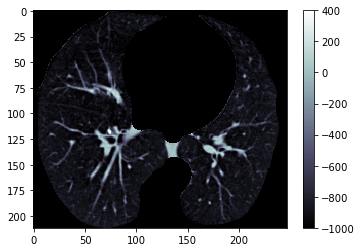
\includegraphics[height=90px]{figures/nodule_seg_pred_1.png} &
  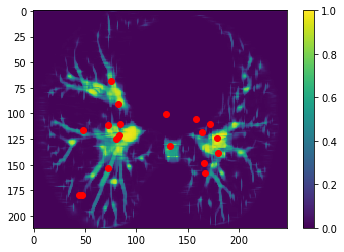
\includegraphics[height=90px]{figures/nodule_seg_pred_2.png} &
  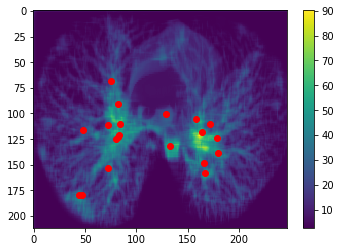
\includegraphics[height=90px]{figures/nodule_seg_pred_3.png} \\
  (a) & (b) & (c) \\
  \end{tabular}
  \caption{An example of nodule segmentation and nodule candidate prediction on the DSB-17 dataset. (a) A slice of the CT scan image along $z$-axis. (b) The predicted nodule probability on every pixels of that slice. The red dots show the centroids of the 20 nodule candidates projected onto that slice. (c) The sum of nodule probabilities along $z$-axis. The red dots show the $x$ and $y$ coordinates of the centroids of the top-20 nodule candidates.}
  \label{fig:nodule_segmentation_cluster}
\end{figure}

\subsection{Lung cancer classification over nodule clusters}
After obtaining the top-20 nodule candidates in each patient's CT scan image on the DSB-17 dataset, we cropped a 3D cubical region centered at the centroid of each nodule candidate, and used the 3D convolutional neural network with the same architecture as described in Table \ref{tab:convnet_1} to obtain a cancer score on each of the 20 nodule candidates. Here, we also need to trade-off for memory constraints: to make the network fit in the GPU memory of Nvidia K40, we restricted the cubical size to be 32mm by 32mm by 32mm.

As the nodule probability at each voxel can be useful to detect cancer, we used it together with the HU values as inputs to the network. During training, we feed the 20 nodules into the network at the same time to obtain 20 cancer scores on the nodule candidates. For each patient, the network output is a 20 dimensional vector, and the input to the network is (20, 32, 32, 32, 2) where the first dimension 20 corresponds to the 20 nodule candidates, and the last dimension 2 corresponds to the two image channels (containing both the HU values and the nodule probability at each location). We took the maximum of the 20 scores to be the cancer score for each patient. The rationale of taking the maximum is that the patient has cancer as long as one of the nodules is cancerous, so the patient-level risk should be the highest risk among the nodules.

This 3D convolutional neural network was trained on cancer/non-cancer labels on the DSB-17 training set. During training, we followed the same setting as in Sec. \ref{sec:method1} and used the sigmoid cross entropy loss in Eqn. \ref{eqn:loss} on the patient-level scores. In this way, we achieved a loss of 0.55 and an accuracy of 76.7\% on the DSB-17 test set (after the challenge deadline), which is comparable the top-50 winners of the Data Science Bowl 2017.

\section{Conclusion}
In this project, we have addressed the challenging lung cancer detection problem with deep convolutional neural networks, and have tried different approaches to solve this task. To address the data limitation and overfitting issues in our first model, we used the LUNA-16 dataset as external training data and developed another classification method. In our second method, we first trained U-Net models on LUNA-16 data for nodule segmentation and predicted top nodule candidates on the DSB-17 dataset, then built a 3D convolution neural network and used the nodule probability together with the HU values of the nodule candidates for cancer/non-cancer classification. Our final model achieves reasonable performance on the DSB-17 dataset.

%In our future work, we would like to further investigate other approaches including: 1) instead of having a separate 2D U-Net for nodule segmentation and a 3D network for cancer prediction, use one 3D convolutional network with two branches on the top for joint nodule segmentation in LUNA-16 and cancer prediction in DSB-17, in order to better utilize the external LUNA-16 data; 2) use multi-GPU training and data parallelism to address the computation cost and memory limitation issue, and increase our batch size and speed up our training process; 3) investigate whether and how we can benefit from other existing convolutional neural network architectures such as VGG \cite{simonyan2014very}, Inception \cite{szegedy2015going} or ResNet \cite{he2016deep} in computer vision.

{\small
\bibliographystyle{unsrt}
\bibliography{references}
}


\end{document}
